\chapter{\textbf{Estudo de Caso}}
Este capítulo visa demonstrar como desenvolver uma aplicação com suporte à \ac{PWA}. Basicamente o app consiste em 3 telas. Será apresentada uma aplicação que utiliza alguns recursos de uma \ac{PWA}, como, funcionamento \textit{offline}, câmera do dispositivo, localização atual, notificações e \textit{background sync}. Para isso foi utilizado algumas ferramentas como \textit{Firebase}, \textit{Workbox} e \textit{IndexedDB}.

\section{Ferramentas Utilizadas}
\subsection{Firebase}
De acordo com \cite{firebase} "O Firebase é uma plataforma do Google que contém várias ferramentas e uma excelente infraestrutura para ajudar desenvolvedores web e mobile a criar aplicações de alta qualidade e performance". Para o desenvolvimento do app, serão utilizados alguns recursos disponibilizados pelo firebase:

\begin{itemize}
	\item \textbf{Realtime Database}: Banco de dados \textit{NoSQL} hospedado em nuvem.
	\item \textbf{Storage}: Banco de dados utilizado para guardar arquivos de mídia, como imagens, vídeos e áudio.
	\item \textbf{Notifications}: Serviço de envio de notificações para usuários conectados.
\end{itemize}

\subsection{IndexedDB}
O \textit{indexedDB} é um banco de dados disponibilizado pelo \textit{browser}, segundo \cite{indexdb} "\textit{IndexedDB} é uma \ac{API} para armazenamento \textit{client-side} de quantidades significantes de informações e buscas com alta performance por índices". \textit{IndexedDB} é a solução para grande porção de dados estruturados.

\subsection{Workbox}
O \textit{workbox} é uma ferramenta, que vai nos ajudar a manipular, de forma mais simples, o \textit{service worker} da aplicação. Segundo \cite{workbox} "O \textit{workbox} é um conjunto de bibliotecas e módulos que facilitam o armazenamento em \textit{cache} e aproveitam ao máximo os recursos usados para criar uma \ac{PWA}".

\section{Conhecendo o Aplicativo}
Para esse projeto foi desenvolvido um aplicativo que realiza postagens. Cada uma dessas postagem deve possuir além da  imagem, uma descrição e a localização de onde foi realizado tal evento. O aplicativo desenvolvido têm três telas:
\begin{itemize}
	\item \textbf{Tela Inicial}: É  apresentação do aplicativo, ela reúne todas as postagens feitas pelos os usuários, e um botão de ação, para criar uma nova postagem no aplicativo. Como é visto na 
	\autoref{telaInicial}.
	\begin{figure}[!htpb]
		\centering
		\caption{Tela Inicial}
		\frame{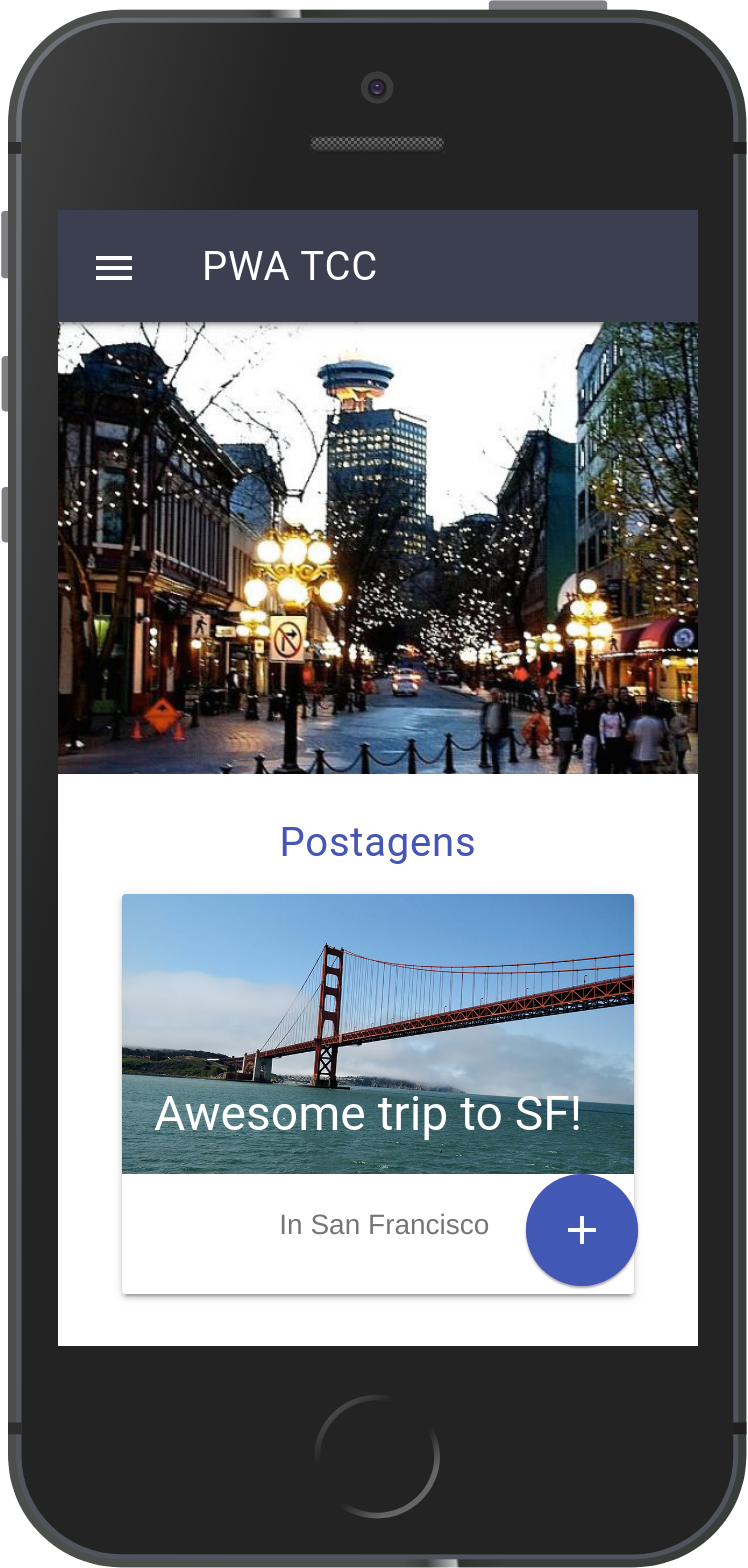
\includegraphics[scale=0.20]{images/tela_inicial.png}}\\
		{\footnotesize Fonte: (Elaborado Pelo Autor, 2019)}
		\label{telaInicial}
	\end{figure}

\newpage
	\item \textbf{Tela de Criação de Postagens}: A \autoref{telaDePost} mostra como é a tela que possibilita ao usuário criar uma postagem.
	\begin{figure}[!htpb]
		\centering
		\caption{Tela de Criação de Post}
		\frame{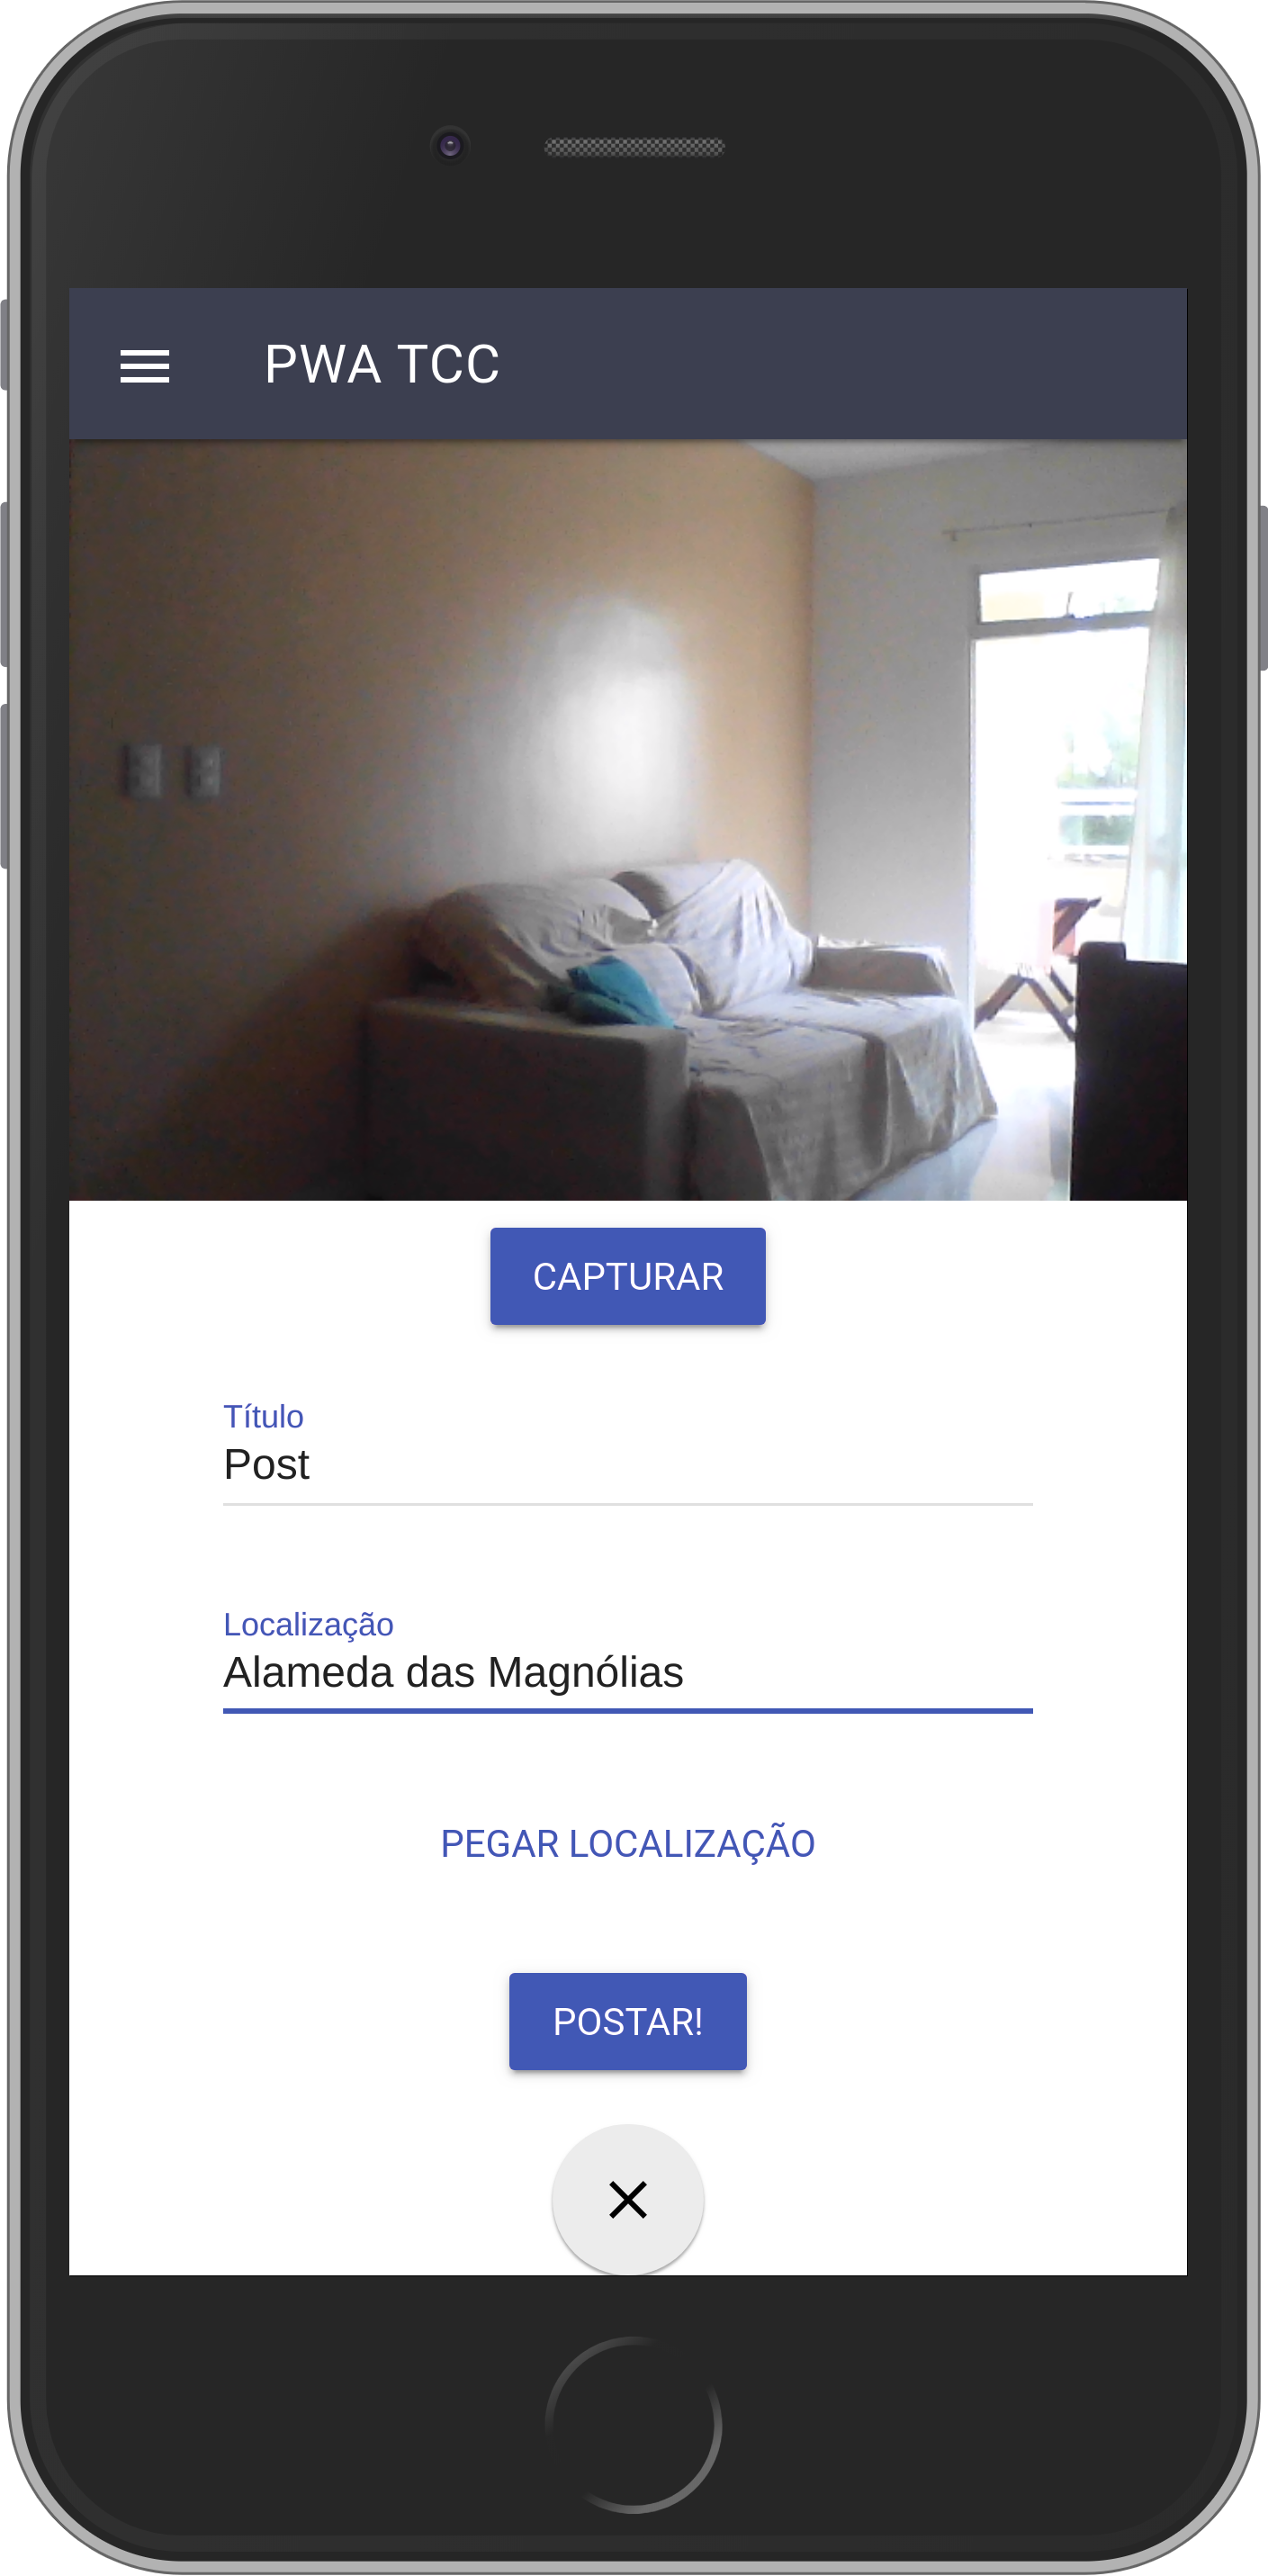
\includegraphics[scale=0.07]{images/tela_post.png}}\\
		{\footnotesize Fonte: (Elaborado Pelo Autor, 2019)}
		\label{telaDePost}
	\end{figure}
	
	\item \textbf{Tela de Ajuda}: É uma página para auxiliar o usuário na navegação do aplicativo. Ainda existem botões de ação que simulariam o entrar em contato com a equipe de SAC, como mostrado na \autoref{telaDeAjuda}.
	\begin{figure}[!htpb]
		\centering
		\caption{Tela de Ajuda}
		\frame{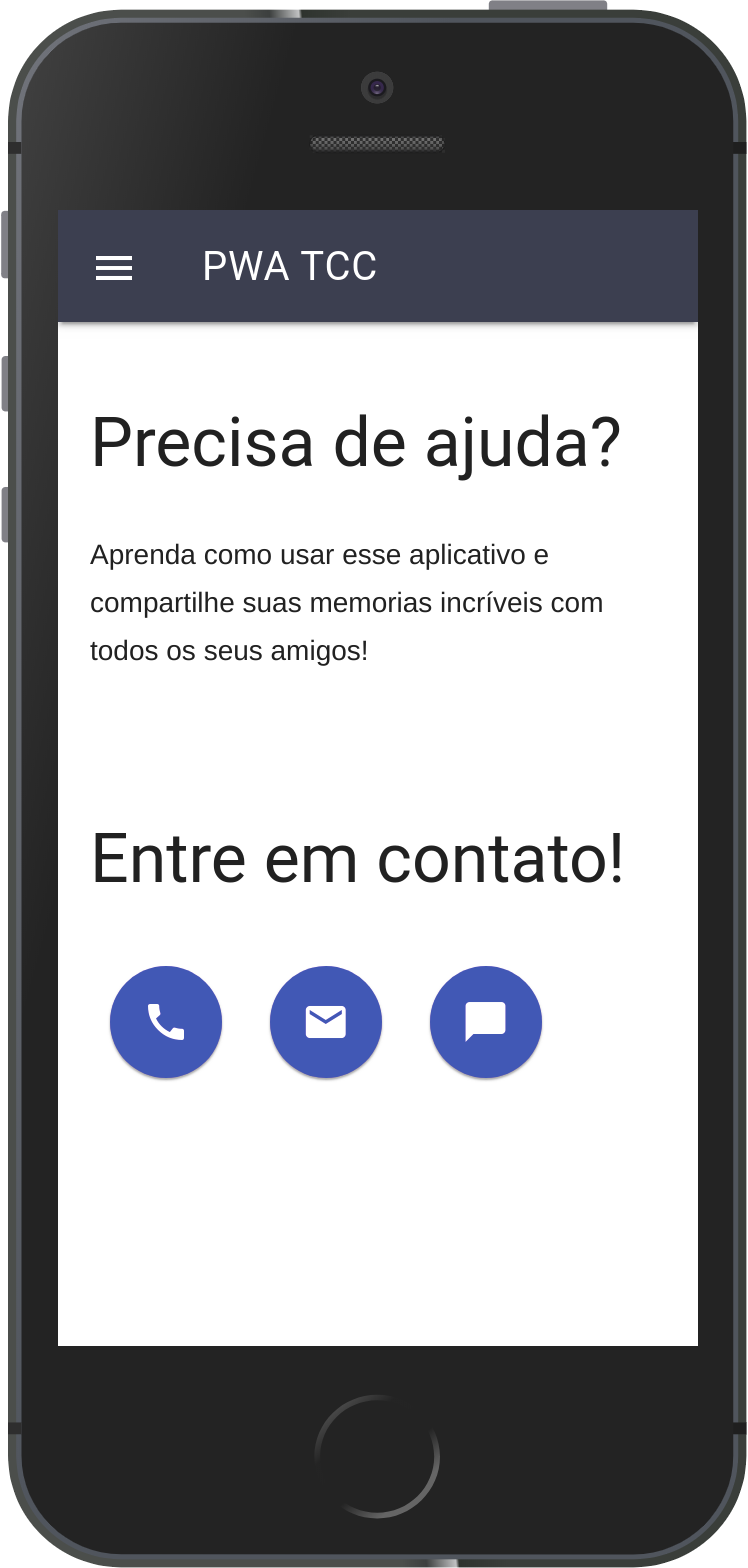
\includegraphics[scale=0.14]{images/tela_ajuda.png}}\\
		{\footnotesize Fonte: (Elaborado Pelo Autor, 2019)}
		\label{telaDeAjuda}
	\end{figure}
\end{itemize}

\section{Configurações Inicias Do Aplicativo com PWA}

\subsection*{Adicionando suporte à PWA}
 Para o aplicativo desenvolvido usar recursos PWA, tem-se que adicionar um  arquivo de configuração do \textit{Service Worker}.

\subsection{Arquivo de Manifesto}
O manifesto da nossa aplicação é configurado por meio de um arquivo de texto, onde possibilita adicionar informações relevantes sobre o aplicativo. Com o arquivo de manifesto configurado nossa aplicação agora pode ser adicionada a tela inicial \cite{manifestfile}. Abaixo a \autoref{f_c4_pwa_custom} que ilustra isso:

\begin{figure}[!htpb]
	\centering
	\caption{Adicionando App}
	\frame{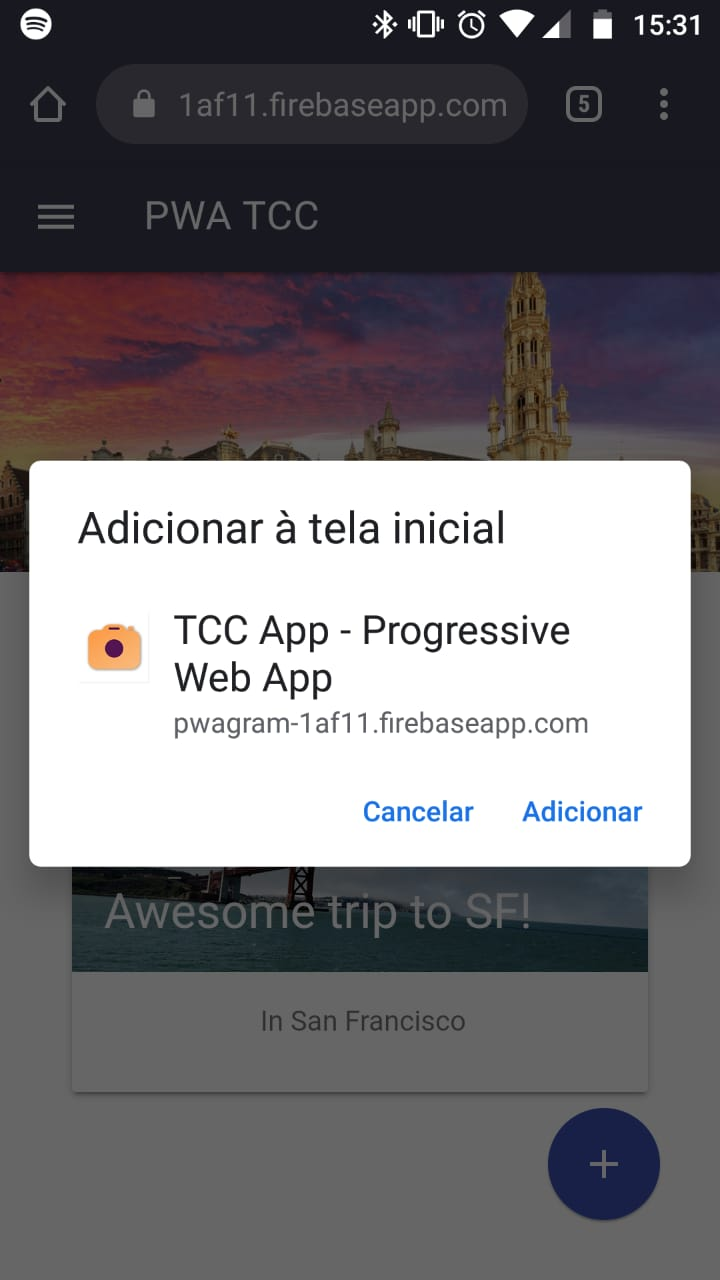
\includegraphics[scale=0.2]{images/pwa_add.jpeg}}\\
	{\footnotesize Fonte: (Elaborado Pelo Autor, 2019)}
	\label{f_c4_pwa_custom}
\end{figure}

E para exemplificar, no \autoref{lst:arquivoManifest} abaixo é mostrado como o manifesto da aplicação ficou configurado:

\newpage

\begin{lstlisting}[frame=single,label=lst:arquivoManifest,caption=Arquivo Manifesto, basicstyle=\footnotesize,]
{
  "name": "TCC App - Progressive Web App",
   "short_name": "PWA TCC",
   "icons": [
 {
   "src": "/src/images/icons/app-icon-48x48.png",
   "type": "image/png",
   "sizes": "48x48"
  },
...
],
"start_url": "/index.html",
"scope": ".",
"display": "standalone",
"orientation": "portrait-primary",
"background_color": "#fff",
"theme_color": "#3c3f50",
"description": "A app, implementing a lot of PWA features.",
"dir": "ltr",
"lang": "en-US"
}
\end{lstlisting}
 \vspace{-0.75cm}
\begin{center}
	\captionof*{lstlisting}{Fonte: (Elaborado Pelo Autor, 2019)}
\end{center}

\subsection{Service Worker}
Como o \textit{service worker} é um \textit{script} do navegador que executa em segundo plano. No primeiro momento vamos apenas configura-lo para fazer cache de alguns recursos úteis a nossa aplicação, como, arquivos \textit{javascript}, css, imagens e páginas html do aplicativo. Para configurar o \textit{service worker}, será criado um arquivo \textit{javascript}, que utilizará uma biblioteca externa chamada \textit{workbox}. O \textit{Workbox} nós ajudará a configurar o \textit{service worker} de maneira mais fácil, já que ele abstrai, muito código \cite{workbox}. O \autoref{lst:serviceWoker} mostra a configuração inicial do  \textit{service worker}.

\newpage

\begin{lstlisting}[frame=single,label=lst:serviceWoker,caption=Service Worker, basicstyle=\footnotesize]
workboxSW.router.registerRoute(:googleapis|gstatic)\.com.
,workboxSW.strategies.staleWhileRevalidate({
  cacheName: 'google-fonts',
  cacheExpiration: {
   maxEntries: 3,
   maxAgeSeconds: 60 * 60 * 24 * 30
  }
}));

workboxSW.router.registerRoute('https://cdnjs.cloudflare.com/ajax/libs/material-design-lite/1.3.0/material.indigo-pink.min.css', workboxSW.strategies.staleWhileRevalidate({
 cacheName: 'material-css'
}));

workboxSW.precache([{
    "url": "favicon.ico",
    "revision": "2cab47d9e04d664d93c8d91aec59e812"
  },
  {
    "url": "index.html",
    "revision": "df4415e7f962b5b6025142af8109f6d2"
  },
  {
    "url": "manifest.json",
    "revision": "cbd4ba1a23f99eb419b91b68d7591d3c"
  },
  {
    "url": "offline.html",
    "revision": "89c91dd62199aa07afc6b6d1ca0db9d1"
  },
  ...
]);

\end{lstlisting}

\vspace{-0.75cm}
\begin{center}
\captionof*{lstlisting}{Fonte: (Elaborado Pelo Autor, 2019)}
\end{center}

\section{Recursos Avançados do Service Worker}
\subsection{Cache das Postagens}
Com o \textit{service worker} configurado, um recurso importante do aplicativo é a listagem de postagens, é possível configurar o \textit{service worker}, para fazer o \textit{cache} das postagens a medida que forem sendo carregadas, assim tornando o aplicativo funcional mesmo em modo \textit{offline}. No arquivo de configuração do \textit{service worker}, criaremos um interceptador para a rota de listagem de Postagens e faremos o tratamento para guardar os dados em cache quando necessário. O \autoref{lst:cacheResponse} mostra o código necessário para que isso seja possível:
\begin{lstlisting}[frame=single,label=lst:cacheResponse,caption=Armazendo Post, basicstyle=\footnotesize]
workboxSW.router.registerRoute(`https://${FIREBASE_URL}/posts.json`, function(args) {
return fetch(args.event.request)
.then(function (res) {
var clonedRes = res.clone();
clearAllData('posts')
.then(function () {
return clonedRes.json();
})
.then(function (data) {
for (var key in data) {
writeData('posts', data[key])
}
});
return res;
});
});
\end{lstlisting}

\vspace{-0.75cm}
\begin{center}
	\captionof*{lstlisting}{Fonte: (Elaborado Pelo Autor, 2019)}
\end{center}

Na configuração acima, os dados retornados da requisição, são guardados no \textit{IndexedDB}, na tabela 'posts'. Quando a requisição é retornada, os dados da tabela 'posts' são limpos, para então ser salvos, afim de manter-mos sempre dados validos no \textit{IndexedDB}.

\subsection{Ações Customizadas}
O \textit{service worker} nos permite customizar ações de tratamento, quando nossa aplicação estiver \textit{offline}, e um recurso interessante que será adicionado, é a exibição de uma página customizada, quando o usuário tenta acessar um recurso offline e que ainda não foi cacheado pelo \textit{service worker}, também conhecida como \textit{fallback page} como mostra a \autoref{offline}.

\begin{figure}[!htpb]
	\centering
	\caption{Tela Offline}
	\frame{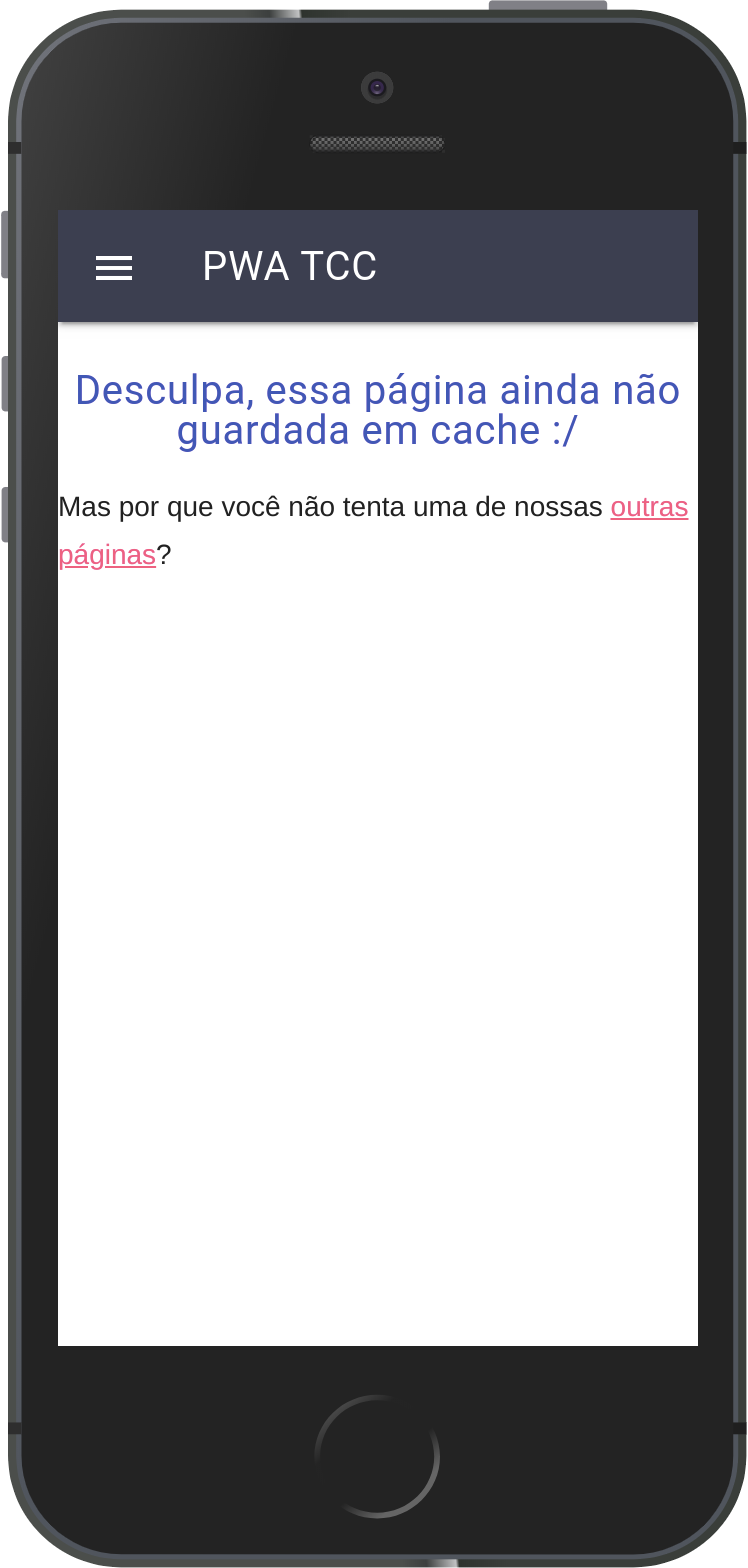
\includegraphics[scale=0.24]{images/pwa_offline.png}}\\
	{\footnotesize Fonte: (Elaborado Pelo Autor, 2019)}
	\label{offline}
\end{figure}

O \autoref{lst:customizado} mostra configuração do \textit{service worker}, para exibir uma página customizada:

\newpage

\begin{lstlisting}[frame=single,label=lst:customizado,caption=Página offline customizada, basicstyle=\footnotesize]
workboxSW.router.registerRoute(function (routeData) {
return (routeData.event.request.headers.get('accept').includes('text/html'));
}, function(args) {
return caches.match(args.event.request)
.then(function (response) {
if (response) {
return response;
} else {
return fetch(args.event.request)
.then(function (res) {
return caches.open('dynamic')
.then(function (cache) {
cache.put(args.event.request.url, res.clone());
return res;
})
})
.catch(function (err) {
return caches.match('/offline.html')
.then(function (res) {
return res;
});
});
}
})
});
\end{lstlisting}

\vspace{-0.75cm}
\begin{center}
	\captionof*{lstlisting}{Fonte: (Elaborado Pelo Autor, 2019)}
\end{center}

\subsection{Sincronização de Dados em Background}
Um recurso interessante que o aplicativo possuí é o envio de postagens, mesmo o usuário estando \textit{offline}, o \textit{service worker}, possui um evento de \textit{sync}, onde nele é possível verificar se o aplicativo está com acesso a internet e realizar uma determinada ação \cite{servicework}. 
\newline{}
Ao cadastrar uma postagem, será salvo no \textit{IndexedDB}, o body da requisição para o servidor na tabela 'sync-posts', após isso será registrado um evento 'sync', com a tag 'sync-new-posts' no \textit{service worker}, para que ele trate-o logo mais. O \autoref{lst:sync} com o código das configurações:
\begin{lstlisting}[frame=single,label=lst:sync,caption=Sicronização Em Background, basicstyle=\footnotesize]
if ('serviceWorker' in navigator && 'SyncManager' in window) {
navigator.serviceWorker.ready
.then(function (sw) {
var post = {
id: new Date().toISOString(),
title: titleInput.value,
location: locationInput.value,
picture: picture,
rawLocation: fetchedLocation
};
writeData('sync-posts', post)
.then(function () {
return sw.sync.register('sync-new-posts');
})
.then(function () {
var snackbarContainer = document.querySelector('#confirmation-toast');
var data = {message: 'Seus post foi salvo para a sincronizaacaoo!'};
snackbarContainer.MaterialSnackbar.showSnackbar(data);
})
.catch(function (err) {
console.log(err);
});
});
} else {
sendData();
}
\end{lstlisting}
\vspace{-0.75cm}
\begin{center}
	\captionof*{lstlisting}{Fonte: (Elaborado Pelo Autor, 2019)}
\end{center}


Para o \textit{service worker} tratar o evento que acabou de ser transmitido, é necessário implementar uma função. Para isso verificaremos se o evento transmitido terá a tag 'sync-new-posts', que foi passada previamente, e assim podemos tratar os dados da forma que quisermos, nesse caso, vai ser chamada os dados do \textit{IndexedDB}, referente a tabela 'sync-posts' e enviaremos os dados para o servidor \textit{Firebase}, e por fim, limpamos os dados da tabela 'sync-posts', que acabaram de ser salvos. A seguir o código da função implementada é mostrada no \autoref{lst:limparDados}:

\begin{lstlisting}[frame=single,label=lst:limparDados,caption=Limpando Dados, basicstyle=\footnotesize]
self.addEventListener('sync', function(event) {
console.log('[Service Worker] Background syncing', event);
if (event.tag === 'sync-new-posts') {
console.log('[Service Worker] Syncing new Posts');
event.waitUntil(
readAllData('sync-posts')
.then(function(data) {
for (var dt of data) {
var postData = new FormData();
postData.append('id', dt.id);
postData.append('title', dt.title);
postData.append('location', dt.location);
postData.append('rawLocationLat', dt.rawLocation.lat);
postData.append('rawLocationLng', dt.rawLocation.lng);
postData.append('file', dt.picture, dt.id + '.png');
fetch(`https://${FIREBASE_FUNCTION_URL}/storePostData`, {
method: 'POST',
body: postData
})
.then(function(res) {
console.log('Sent data', res);
if (res.ok) {
res.json()
.then(function(resData) {
deleteItemFromData('sync-posts', resData.id);

\end{lstlisting}
\vspace{-0.75cm}
\begin{center}
	\captionof*{lstlisting}{Fonte: (Elaborado Pelo Autor, 2019)}
\end{center}

\subsection{Notificações}
Notificações é uma ferramenta importante para informar o usuário sobre um determinado evento, tendo isso em vista, o aplicativo desenvolvido vai enviar notificações para os usuários quando for criada uma nova postagem. Para a criação do fluxo de notificação foi usado o \textit{Firebase} e configurações no arquivo do \textit{service worker}. Em um primeiro momento é necessário verificar se o usuário deseja receber notificações, por isso, o aplicativo possui um botão que habilita as notificações. Como mostra a figura \autoref{notificacao}.

\begin{figure}[!htpb]
	\centering
	\caption{Habilitar Notificações}
	\frame{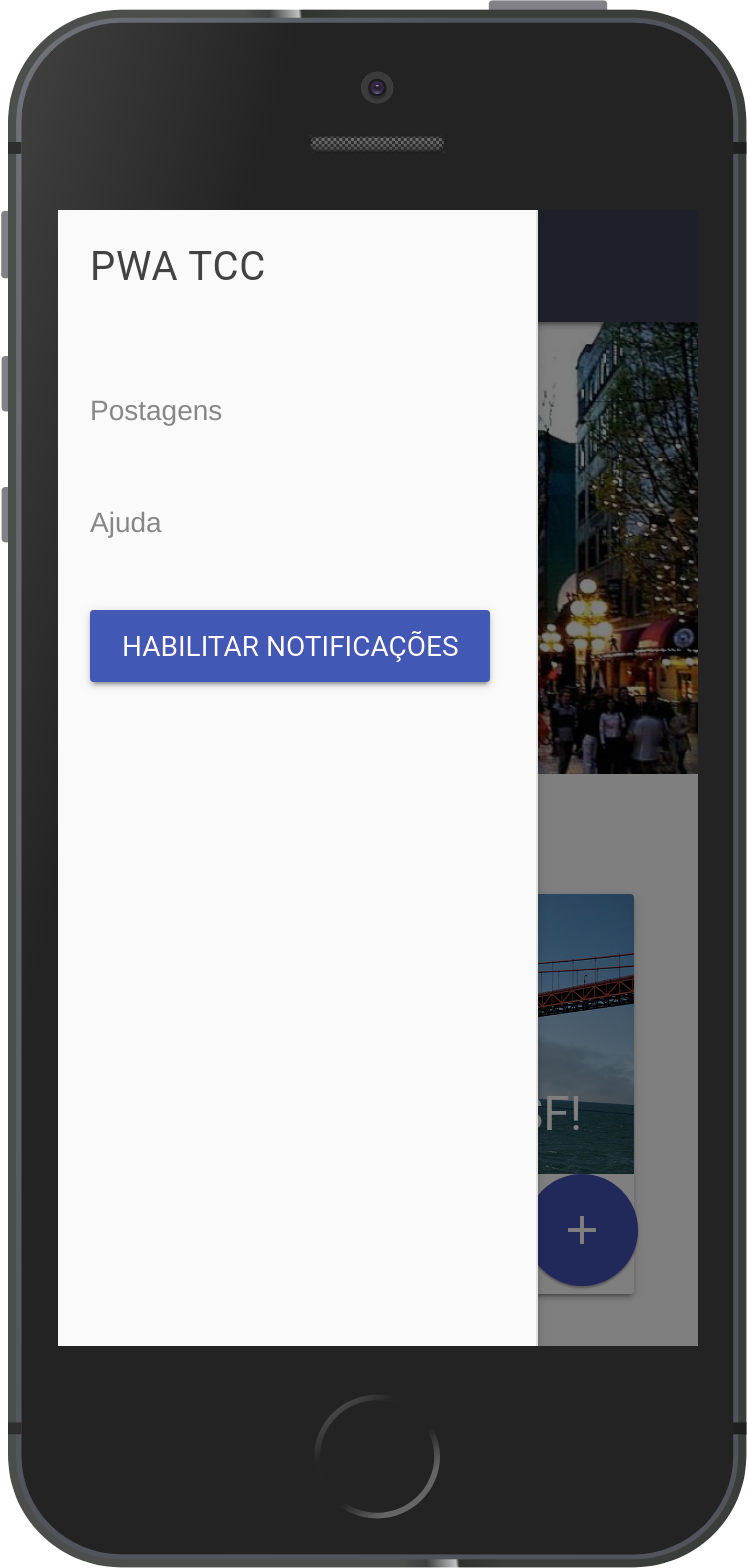
\includegraphics[scale=0.15]{images/pwa_notification.png}}\\
	{\footnotesize Fonte: (Elaborado Pelo Autor, 2019)}
	\label{notificacao}
\end{figure}

Este botão só estará disponível se o browser possuir suporte as notificações, para isso foi adicionado uma verificação, em que esconde o botão caso as notificações não estiverem disponíveis. O \autoref{lst:notificacoes} mostra a lógica para que isso aconteça.

\begin{lstlisting}[frame=single,label=lst:notificacoes,caption=Verificando suporte notificações, basicstyle=\footnotesize]
if ('Notification' in window && 'serviceWorker' in navigator) {
for (var i = 0; i < enableNotificationsButtons.length; i++) {
enableNotificationsButtons[i].style.display = 'inline-block';
enableNotificationsButtons[i].addEventListener('click', askForNotificationPermission);
}
}
\end{lstlisting}
\vspace{-0.75cm}
\begin{center}
	\captionof*{lstlisting}{Fonte: (Elaborado Pelo Autor, 2019)}
\end{center}

\newpage
O \textit{browser} tendo suporte as notificações, é necessário a permissão do usuário para podermos utiliza-las. Como mostra o \autoref{lst:permissao}.

\begin{lstlisting}[frame=single,label=lst:permissao,caption=Pedindo permissão ao usuário, basicstyle=\footnotesize]
function askForNotificationPermission() {
Notification.requestPermission(function(result) {
console.log('User Choice', result);
if (result !== 'granted') {
console.log('No notification permission granted!');
} else {
configurePushSub();
}
});
}
\end{lstlisting}
\vspace{-0.75cm}
\begin{center}
	\captionof*{lstlisting}{Fonte: (Elaborado Pelo Autor, 2019)}
\end{center}

O usuário dando permissão para o aplicativo usar as notificações, podemos configurar-las e criar uma inscrição no \textit{Firebase}, essa inscrição vai auxiliar no envio das notificações, como uma identificação para o dispositivo do usuário e enviar a notificação para eles. Para essa ação, foi criada uma função que verifica se o dispositivo já possui uma inscrição,conforme pode ser visto no Quadro 9.


\begin{lstlisting}[frame=single,label=lst:inscricao,caption=Configurando Push Notifications, basicstyle=\footnotesize]
function configurePushSub() {
if (!('serviceWorker' in navigator)) return;
var reg;
navigator.serviceWorker.ready
.then(function(swreg) {
reg = swreg;
return swreg.pushManager.getSubscription();
})
.then(function(sub) {
if (sub === null) {
// Create a new subscription
var convertedVapidPublicKey = urlBase64ToUint8Array(PUBLIC_KEY);
return reg.pushManager.subscribe({
userVisibleOnly: true,
applicationServerKey: convertedVapidPublicKey
});
}
})
.then(function(newSub) {
return fetch(`https://${FIREBASE_URL}/subscriptions.json`, {
method: 'POST',
headers: {
'Content-Type': 'application/json',
'Accept': 'application/json'
},
body: JSON.stringify(newSub)
})
})
.then(function(res) {
if (res.ok) {
displayConfirmNotification();
}
})
.catch(function(err) {
console.log(err);
});
}
\end{lstlisting}
\vspace{-0.75cm}
\begin{center}
	\captionof*{lstlisting}{Fonte: (Elaborado Pelo Autor, 2019)}
\end{center}


\newpage
No retorno da requisição para o \textit{Firebase}, se tudo ocorrer bem, é chamada uma função que exibe para o usuário uma notificação, pré configurada, conforme exibido no Quadro 10..
\begin{lstlisting}[frame=single,label=lst:pushNotificacao,caption= Notificação Pré configurada, basicstyle=\footnotesize]
function displayConfirmNotification() {
if ('serviceWorker' in navigator) {
var options = {
body: 'You successfully subscribed to our Notification service!',
icon: '/src/images/icons/app-icon-96x96.png',
image: '/src/images/sf-boat.jpg',
dir: 'ltr',
lang: 'en-US', // BCP 47,
vibrate: [100, 50, 200],
badge: '/src/images/icons/app-icon-96x96.png',
tag: 'confirm-notification',
renotify: true,
actions: [
{ action: 'confirm', title: 'Okay', icon: '/src/images/icons/app-icon-96x96.png' },
{ action: 'cancel', title: 'Cancel', icon: '/src/images/icons/app-icon-96x96.png' }
]
};
navigator.serviceWorker.ready
.then(function(swreg) {
swreg.showNotification('Successfully subscribed!', options);
});
}
}
\end{lstlisting}
\vspace{-0.75cm}
\begin{center}
	\captionof*{lstlisting}{Fonte: (Elaborado Pelo Autor, 2019)}
\end{center}

\newpage
A \autoref{configuracaoNotificacao}, mostra  o exemplo, de como será exibido a notificação:

\begin{figure}[!htpb]
	\centering
	\caption{Notificação Pré Configurada}
	\frame{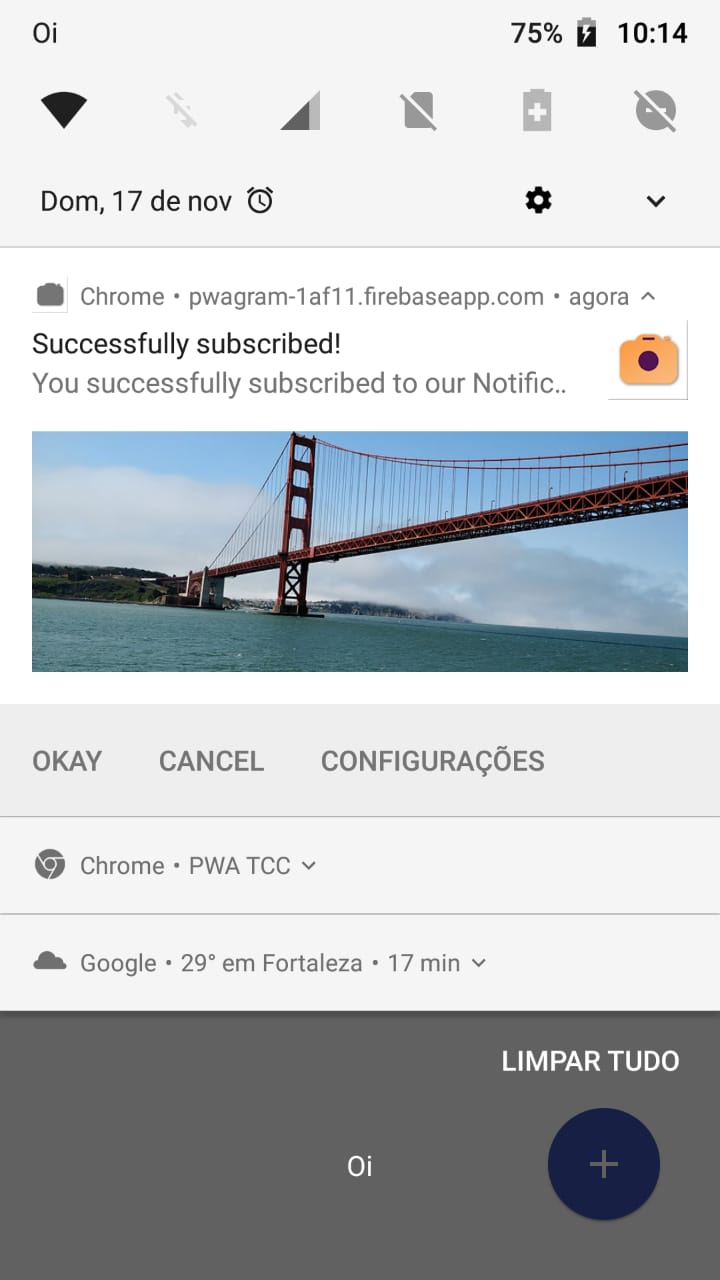
\includegraphics[scale=0.15]{images/pwa_default_notification.jpeg}}\\
	{\footnotesize Fonte: (Elaborado Pelo Autor, 2019)}
	\label{configuracaoNotificacao}
\end{figure}

Por fim, para exibir as notificações, é necessário, configurar o service worker. O \textit{service worker} possui o evento 'push', onde é configurada uma função para o tratamento das notificações, conforme mostra o \autoref{lst:notificacaoPersonalixada}.
\begin{lstlisting}[frame=single,label=lst:notificacaoPersonalixada,caption= Notificação personalizada, basicstyle=\footnotesize]
self.addEventListener('push', function(event) {
console.log('Push Notification received', event);
var data = {title: 'New!', content: 'Something new happened!', openUrl: '/'};
if (event.data) data = JSON.parse(event.data.text());
var options = {
body: data.content,
icon: '/src/images/icons/app-icon-96x96.png',
badge: '/src/images/icons/app-icon-96x96.png',
data: {
url: data.openUrl
event.waitUntil(self.registration.showNotification(data.title, options));
\end{lstlisting}
\vspace{-0.62cm}
\begin{center}
	\captionof*{lstlisting}{Fonte: (Elaborado Pelo Autor, 2019)}
\end{center}